Consta de dos clases Clave y Usuario las cuales ambas se 
definen en usuario.hpp y se implementan en usuario.cpp, como hemos 
comentado anteriormente.
\subsection{Clase Clave}
Esta clase se va a crear mediante una Cadena que alojará una contraseña que cifraremos.
El constructor recibirá una cadena caracteres de bajo nivel \texttt{const char *} que contendrá la contraseña sin cifrar.
Declaramos las clases de excepción \textbf{Clave::Incorrecta} que devolverá la razón por la que se ha llevado a cabo la excepción serán (CORTA y ERROR\_CRYPT), esta clase de excepción devolverá el atributo correspondiente mediante el observador \texttt{razon()}.

Tendremos un observador llamado \texttt{clave()} que devuelve la contraseña cifrada almacenada.

Por último encontramos el método \texttt{verifica()} que recibirá como parámetro una cadena de caracteres de bajo nivel (contraseña sin cifrar) y devuelve un booleano si se corresponde con la contraseña almacenada, en este caso devuelve \textbf{true}, si no \textbf{false}.

\subsection{Clase Usuario}
La clase Usuario contrendrá estos atributos:
\begin{itemize}
    \item 4 Cadenas que serán: identificador, nombre, apellido y dirección (por este orden).
    \item Una contraseña que será de tipo Clave.
    \item Un diccionario de tarjetas público (\texttt{std::map<Numero,Tarjeta*>}), que se tiene que llamar Tarjetas.
    \item El contenido del carrito, que será un diccionario de artículos junto con la cantidad de los mismos (\texttt{std::unordered\_map<Articulo*,unsigned>}) que es público y se tiene que llamar Articulos.
\end{itemize}

El constructor recibirá 5 parámetros que son: identificador, nombre, apellido, dirección y clave.
Este constructor debe de comprobar que el Usuario se crea correctamente:
\begin{itemize}
    \item Comprueba que el identificador no esté repetido, si no se lanza la excepción \textbf{Usuario::Id\_duplicado}, que devuelve el atributo a través del observador \texttt{idd()}.
    \item Un Usuario NO puede crearse por copia a través de otro (ni constructor ni operador de asignción por copia.)
\end{itemize}

La clase tendrá varios métodos observadores: \texttt{id()}, \texttt{nombre()}, \texttt{apellido()}, \texttt{direccion()}, \texttt{tarjetas()} y \texttt{compra()}. No devolvemos la clave.

Como la clase Usuario y Tarjeta están relacionadas entre sí, vamos a declarar el método \texttt{es\_titular\_de()} y \texttt{no\_es\_titular\_de()} que recibe como parámetro la tarjeta y que se encargarán de crear y eliminar los enlaces de las clases.

A la hora de destruir una tarjeta primero la tenemos que desvincular de su titular, por eso llamará al método \textbf{Tarjeta::anula\_titular()}

La clase Usuario y Articulo se relacionan mediante una asociación undireccional mediante el método \texttt{compra()}, que será una sobrecarga del observador, pero este va a recibir dos parámetros (Articulo y cantidad). Si la cantidad que se introduce es 0, se elimina, si es mayor que 0, se añade al carrito.
Con este método sobrecargado podemos eliminar Articulos de la compra, pero también tenemos el método \texttt{vaciar\_carro()} que eliminará todos los artículos del carro.

Mediante el observador \texttt{n\_articulos()} devolvemos el número de articulos que contiene el carrito.

Vamos a sobrecargar el operdor de inserción en flujo \texttt{operator <<} para mostrar los datos del Usuario con el formato:

    \textit{identificador [clave cifrada] nombre apellidos}\\
    \textit{dirección}\\
    \textit{Tarjetas:}\\
    \textit{\textless lista de tarjetas\textgreater}


Por último, vamos a definir otro método \texttt{mostrar\_carro()} (externa a la clase), para mostrar el contenido del carro en el flujo de salida con el formato:
\begin{center}
    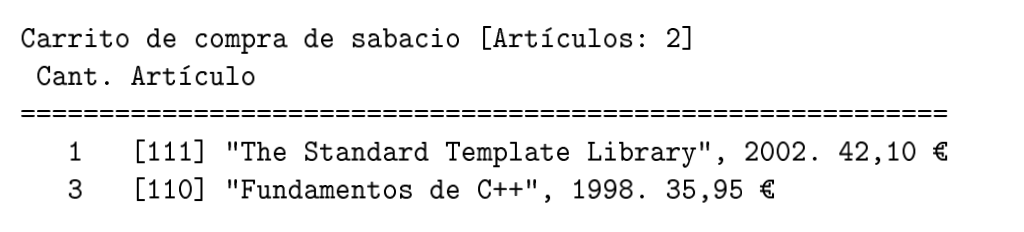
\includegraphics[width=\textwidth]{Pics/P2_3.png}
\end{center}

\newpage
\subsection{Usuario.hpp}
\begin{minted}[breaklines]{C++}
#ifndef USUARIO_HPP
#define USUARIO_HPP

//Inclusión de librerías
#include "../P1/cadena.hpp"
#include "tarjeta.hpp"
#include "articulo.hpp"
#include <random>
#include <map>
#include <unordered_map>
#include <unordered_set>
#include <iomanip>

//Declaraciones adelantadas
class Numero;
class Tarjeta;
/*-----Clase Clave-----*/
class Clave{
    public:
        typedef enum {CORTA,ERROR_CRYPT}Razon;
        Clave(const char*);

        //observador de la clase
        inline Cadena clave()const {return password_;}
        bool verifica(const char* )const;
        //Clase de la excepción
        class Incorrecta{
            Razon razon_;
            public:
                Incorrecta(const Razon& r):razon_(r){};
                const Razon& razon()const{return razon_;}
        };
    private:
        Cadena password_;
};

/*-----Clase Usuario-----*/
class Usuario{
    public:
        typedef std::map<Numero,Tarjeta*> Tarjetas;
        typedef std::unordered_map<Articulo*,unsigned int>Articulos;

        Usuario(const Cadena& ,const Cadena& , const Cadena& , const Cadena& , const Clave& );
        //eliminamos el ctor de copia y el operador de asignacion
        Usuario(const Usuario&)=delete;
        Usuario operator = (const Usuario&)=delete;
        //métodos observadores
        inline Cadena id()const noexcept{return identificador_;}
        inline Cadena nombre()const noexcept{return nombre_;}
        inline Cadena apellidos()const noexcept{return apellidos_;}
        inline Cadena direccion()const noexcept{return direccion_;}
        inline const Tarjetas& tarjetas()const noexcept{return tarjetas_;}
        inline const Articulos& compra()const noexcept{return articulos_;}
        
        //metodos de la asociacion con clase Tarjeta
        void es_titular_de(Tarjeta&) noexcept;
        void no_es_titular_de(Tarjeta&) noexcept;
        //métodos de la asociación unidireccional con Articulos
        void compra( Articulo&, size_t cantidad = 1) noexcept;
        inline void vaciar_carro() noexcept {articulos_.clear();}
        inline size_t n_articulos()const noexcept {return articulos_.size();}

        //destructor de la clase usuario
        ~Usuario();
        //Clase de la excepcion
        class Id_duplicado{
            Cadena id_;
            public:
                Id_duplicado(const Cadena& id):id_(id){};
                const Cadena& idd()const{return id_;}
        };
        friend std::ostream& operator <<(std::ostream& , const Usuario&)noexcept;
    private:
        const Cadena identificador_, nombre_,apellidos_,direccion_;
        Clave clave_;
        Tarjetas tarjetas_;
        Articulos articulos_;
        static std::unordered_set<Cadena> usuario_; //conjunto de usuarios no repetidos del programa
};
void mostrar_carro(std::ostream& , const Usuario&);
#endif // !USUARIO_HPP
    
    
\end{minted}

\subsection{Usuario.cpp}
\begin{minted}[breaklines]{C++}
#include "usuario.hpp"
#include <unistd.h> //crypt()

//Inicialización del conjunto global de usuarios
std::unordered_set<Cadena>Usuario::usuario_;
/*---Clase Clave----*/
Clave:: Clave(const char* c){
    //Comprobamos tamaño de la clave
    if(strlen(c)<5){
        throw Incorrecta(Razon::CORTA);
    }
    else{
        //Encriptamos la clave nueva
        const char* valores ="abcdefghijklmnopqrstuvwxyzABCDEFGHIJKLMNOPQRSTUVWXYZ0123456789./";
        std::random_device random;
        std::uniform_int_distribution<>distribucion(0,63);
        char cifrado[2]={valores[distribucion(random)],valores[distribucion(random)]};
        //comprabamos que el cifrado sea correcto, si no excepción
        if(crypt(c,cifrado)){
            password_ = crypt(c,cifrado);
        }else{
            throw Incorrecta(Razon::ERROR_CRYPT);
        }
    }
}
bool Clave::verifica(const char* clave)const{
    //compara la encriptación de la clave que hemos metido concuerda con una de las claves
    return !(strcmp(crypt(clave, password_.operator const char *()),
                password_.operator const char *()));
}

/*-----Clase Usuario-----*/
Usuario::Usuario(const Cadena& id ,const Cadena& nom, const Cadena& apell ,const Cadena& dir ,const Clave& clave):
    identificador_(id),nombre_(nom),apellidos_(apell),direccion_(dir),clave_(clave){
    //Vamos a compromar si el usuario no existe en la lista de usuarios del programa
    if(!usuario_.insert(id).second)throw Usuario::Id_duplicado(id);
}
void Usuario::es_titular_de(Tarjeta& t) noexcept{
    //asosicamos el usuario con la tarjeta
    if(this==t.titular()){
        tarjetas_.insert(std::make_pair(t.numero(),&t));
    }
}

void Usuario::no_es_titular_de(Tarjeta& t) noexcept{
    //desvinculamos el usuario con la tarjeta
    t.anula_titular();
    tarjetas_.erase(t.numero());
}

void Usuario::compra( Articulo& art, size_t cantidad) noexcept{
    //si la cantidad del articulo es > 0 -> se añade; si no se elimina
    if(cantidad > 0)articulos_[&art]=cantidad; //articulos_.insert(std::make_pair(&art,cantidad));
    else articulos_.erase(&art);
}

Usuario::~Usuario(){
    //Para eliminar al usuario tenemos que desligar todas sus tarjetas y luego
    //eliminarlo
    for(auto i = tarjetas_.begin(); i!=tarjetas_.end();i++){
        i->second->anula_titular();
    }
    usuario_.erase(identificador_);
}
    
void mostrar_carro(std::ostream& output , const Usuario& user){
    output << "Carrito de compra de "<<user.id()<<" [Artículos: "<<user.n_articulos()<<"]\n"
            << "Cant. Artículo"<<std::endl;
    output <<std::setw(95)<<std::setfill('=')<<' '<<std::endl; //estética del formato
    //creamos una variable para tener control del numero de articulos del carro
    int n_art = user.n_articulos();
    while(n_art > 0){
        for(auto i=user.compra().begin();i!=user.compra().end();i++){
            output<<std::setw(4)<<std::setfill(' ')<< i->second
                <<" ["<<(*i->first).referencia()<<"] "<<"\""
                <<(*i->first).titulo()<<"\""<<", "
                <<(*i->first).f_publi().anno()<<". "
                <<std::fixed<<std::setprecision(2)<<(*i->first).precio()<<" €"<<std::endl;
            n_art--;
        }
    }
}
std::ostream& operator <<(std::ostream& output , const Usuario& user)noexcept{
    output << user.id() <<" ["<<user.clave_.clave().operator const char *()<<"] "<<user.nombre()<<" "
    <<user.apellidos()<<"\n"<<user.direccion()<<std::endl;
    output<<"Tarjetas: \n"<<std::endl;
    for(auto i = user.tarjetas().begin(); i!=user.tarjetas().end(); i++)
        output<< *i->second<<std::endl;
    return output;
}
\end{minted}